\chapter{Ergebnisse}
\label{ch:ergebnisse}

\section{Theoretische Modellwerte – keine Messdaten}
Die Werte in Tabelle~\ref{tab:modell} wurden allein mithilfe von
Gleichung~\eqref{eq:pendel} für \(g=\qty{9.81}{\meter\per\second\squared}\)
berechnet. \textbf{Es handelt sich ausdrücklich nicht um experimentell
gewonnene Daten.}

\begin{table}[htbp]
  \centering
  \caption{Rechnerisch erzeugte Demonstrationswerte; keine Messwerte}
  \label{tab:modell}
  \begin{tabular}{S[table-format=1.2] S[table-format=1.3]}
    \toprule
    {Pendellänge \(l\) (\si{\meter})} & {Modellperiode \(T\) (\si{\second})} \\
    \midrule
    0.25 & 1.003 \\
    0.50 & 1.419 \\
    0.75 & 1.737 \\
    1.00 & 2.006 \\
    \bottomrule
  \end{tabular}
\end{table}

\section{Grafische Darstellung}
Abbildung~\ref{fig:modell} veranschaulicht denselben berechneten
Zusammenhang. In einer echten BLL sollten hier eigene Messergebnisse,
Fehlerbalken und gegebenenfalls ein Modellvergleich stehen.

\begin{figure}[htbp]
  \centering
  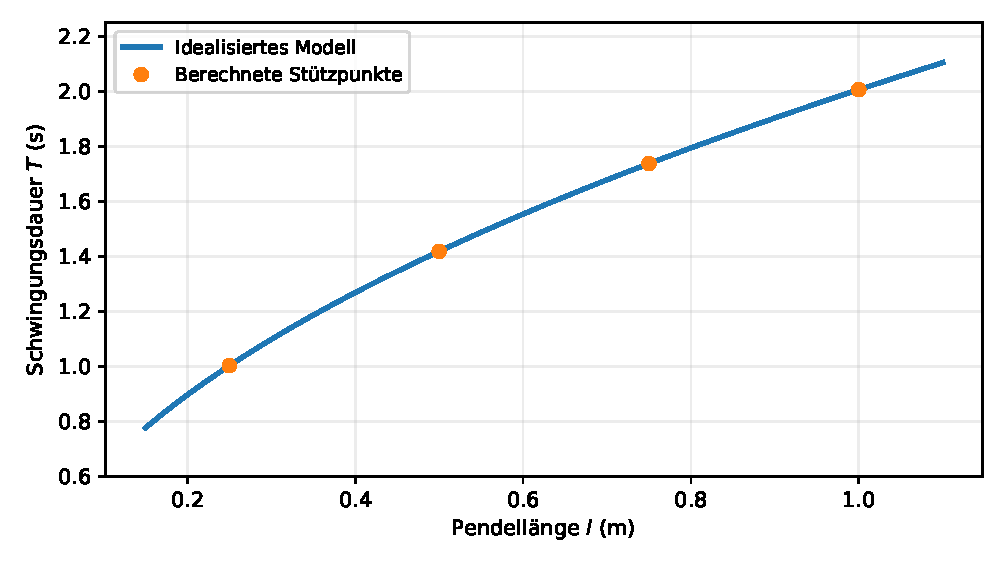
\includegraphics[width=.86\linewidth]{abbildungen/modellkurve.pdf}
  \caption{Theoretische Schwingungsdauer in Abhängigkeit von der Pendellänge
    (eigene Berechnung aus Gleichung~\eqref{eq:pendel})}
  \label{fig:modell}
\end{figure}
